%%%%%%%%%%%%%%%%%%%%%%%%%%%%%%%%%%%%%%%%%
% Jacobs Landscape Poster
% LaTeX Template
% Version 1.1 (14/06/14)
%
% Created by:
% Computational Physics and Biophysics Group, Jacobs University
% https://teamwork.jacobs-university.de:8443/confluence/display/CoPandBiG/LaTeX+Poster
% 
% Further modified by:
% Nathaniel Johnston (nathaniel@njohnston.ca)
%
% This template has been downloaded from:
% http://www.LaTeXTemplates.com
%
% License:
% CC BY-NC-SA 3.0 (http://creativecommons.org/licenses/by-nc-sa/3.0/)
%
%%%%%%%%%%%%%%%%%%%%%%%%%%%%%%%%%%%%%%%%%

%----------------------------------------------------------------------------------------
%	PACKAGES AND OTHER DOCUMENT CONFIGURATIONS
%----------------------------------------------------------------------------------------

\documentclass[final, 14pt]{beamer}

\usepackage[scale=1.24]{beamerposter} % Use the beamerposter package for laying out the poster

\usetheme{confposter} % Use the confposter theme supplied with this template

\setbeamercolor{block title}{fg=Mahogany,bg=white} % Colors of the block titles
\setbeamercolor{block body}{fg=black,bg=white} % Colors of the body of blocks
\setbeamercolor{block alerted title}{fg=white,bg=Mahogany} % Colors of the highlighted block titles
\setbeamercolor{block alerted body}{fg=black,bg=dblue!10} % Colors of the body of highlighted blocks
% Many more colors are available for use in beamerthemeconfposter.sty

%-----------------------------------------------------------
% Define the column widths and overall poster size
% To set effective sepwid, onecolwid and twocolwid values, first choose how many columns you want and how much separation you want between columns
% In this template, the separation width chosen is 0.024 of the paper width and a 4-column layout
% onecolwid should therefore be (1-(# of columns+1)*sepwid)/# of columns e.g. (1-(4+1)*0.024)/4 = 0.22
% Set twocolwid to be (2*onecolwid)+sepwid = 0.464
% Set threecolwid to be (3*onecolwid)+2*sepwid = 0.708

\newlength{\sepwid}
\newlength{\onecolwid}
\newlength{\twocolwid}
\newlength{\threecolwid}
\setlength{\paperwidth}{48in} % A0 width: 46.8in
\setlength{\paperheight}{36in} % A0 height: 33.1in
\setlength{\sepwid}{0.024\paperwidth} % Separation width (white space) between columns
\setlength{\onecolwid}{0.22\paperwidth} % Width of one column
\setlength{\twocolwid}{0.464\paperwidth} % Width of two columns
\setlength{\threecolwid}{0.708\paperwidth} % Width of three columns
\setlength{\topmargin}{-0.5in} % Reduce the top margin size
%-----------------------------------------------------------

\usepackage{graphicx}  % Required for including images

\usepackage{booktabs} % Top and bottom rules for tables

%----------------------------------------------------------------------------------------
%	TITLE SECTION 
%----------------------------------------------------------------------------------------

\title{NBA Predictions}% Poster title

\author{Lee Richardson, Daren Wang, Xiaofeng Yu, Chi Zhang} % Author(s)

\institute{Carnegie Mellon University} % Institution(s)

%----------------------------------------------------------------------------------------

\begin{document}

\addtobeamertemplate{block end}{}{\vspace*{2ex}} % White space under blocks
\addtobeamertemplate{block alerted end}{}{\vspace*{2ex}} % White space under highlighted (alert) blocks

\setlength{\belowcaptionskip}{2ex} % White space under figures
\setlength\belowdisplayshortskip{2ex} % White space under equations

\begin{frame}[t] % The whole poster is enclosed in one beamer frame

\begin{columns}[t] % The whole poster consists of three major columns, the second of which is split into two columns twice - the [t] option aligns each column's content to the top

\begin{column}{\sepwid}\end{column} % Empty spacer column

\begin{column}{\onecolwid} % The first column

%----------------------------------------------------------------------------------------
%	OBJECTIVES
%----------------------------------------------------------------------------------------

\begin{block}{Goals}

\begin{itemize}

  \item The goal of this project was to predict the outcomes of NBA basketball games as accurately as possible

  \item Using game predictions, we can create a distribution of how many games each team is expected to win over the course of a season. 

\end{itemize}

\end{block}

%----------------------------------------------------------------------------------------
%	INTRODUCTION
%----------------------------------------------------------------------------------------

\begin{block}{Introduction}

	

\end{block}

%----------------------------------------------------------------------------------------
% Data
%----------------------------------------------------------------------------------------

\begin{block}{Data}

\begin{itemize}

  \item What's up?

\end{itemize}

\begin{figure}
  \centering
	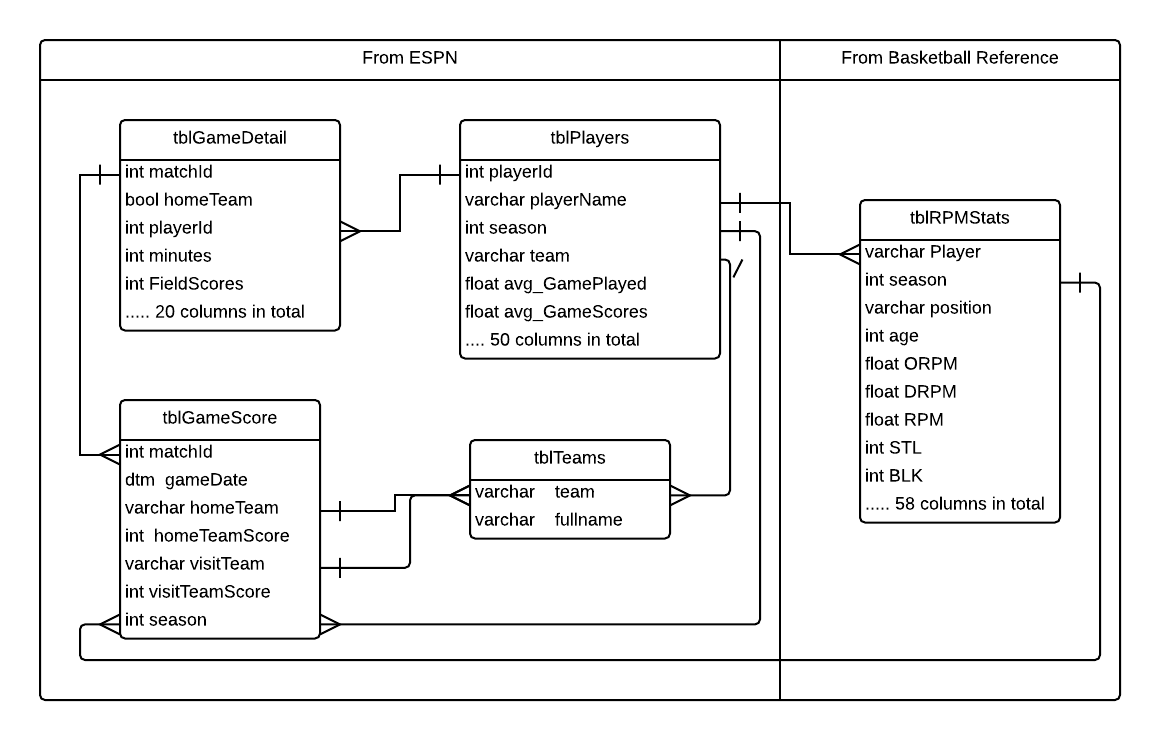
\includegraphics[width=25cm, height=30cm]{sqliteERDiagram.png}
  \caption{Close-up of a gull}
  \label{fig:gull}
\end{figure}

\end{block}

\end{column} % End of the first column

%----------------------------------------------------------------------------------------
% END OF COLUMN ONE
%----------------------------------------------------------------------------------------


\begin{column}{\sepwid}\end{column} % Empty spacer column

\begin{column}{\twocolwid} % Begin a column which is two columns wide (column 2)

\begin{columns}[t,totalwidth=\twocolwid] % Split up the two columns wide column

\begin{column}{\onecolwid}\vspace{-.6in} % The first column within column 2 (column 2.1)

%----------------------------------------------------------------------------------------
%	Data
%----------------------------------------------------------------------------------------

\begin{block}{Features}

  These are the features we used 

\end{block}

%----------------------------------------------------------------------------------------

\end{column} % End of column 2.1

\begin{column}{\onecolwid}\vspace{-.6in} % The second column within column 2 (column 2.2)

%----------------------------------------------------------------------------------------
%	Geography
%----------------------------------------------------------------------------------------

\begin{block}{Algorithms }
\begin{itemize}
\item Must reconcile geographies defined by different entities
\begin{itemize}
\item e.g. ACS SF are available at tract level
\item PUMS data's base level is the PUMA
\end{itemize}
\end{itemize}
\end{block}

%----------------------------------------------------------------------------------------

\end{column} % End of column 2.2

\end{columns} % End of the split of column 2 - any content after this will now take up 2 columns width



\end{column} % End of the second column

%----------------------------------------------------------------------------------------
% END OF THE SECOND COLUMN
%----------------------------------------------------------------------------------------

\begin{column}{\sepwid}\end{column} % Empty spacer column

\begin{column}{\onecolwid} % The third column

%----------------------------------------------------------------------------------------
%	Simulations
%----------------------------------------------------------------------------------------

\begin{block}{Simulations}

  Hey

\end{block}

%----------------------------------------------------------------------------------------
%	CONCLUSION & Future Work
%----------------------------------------------------------------------------------------

\begin{block}{Conclusion}

Yo

\end{block}

%----------------------------------------------------------------------------------------
%	Future Work
%----------------------------------------------------------------------------------------

\begin{block}{Future Work}

\end{block}


%----------------------------------------------------------------------------------------
%	ACKNOWLEDGEMENTS
%----------------------------------------------------------------------------------------

\setbeamercolor{block title}{fg=Mahogany,bg=white} % Change the block title color

\begin{block}{Acknowledgements}

\small{\rmfamily{This research was made possible under NIH Grant MIDAS.  We would also like to thank Carnegie Mellon University's Department of Statistics and the SURE 2014 proram as well as Dr. Bill Eddy for his guidance and support.}} \\

\end{block}

%----------------------------------------------------------------------------------------
%	CONTACT INFORMATION
%----------------------------------------------------------------------------------------

\setbeamercolor{block alerted title}{fg=white,bg=Mahogany} % Change the alert block  colors
\setbeamercolor{block alerted body}{fg=black,bg=dblue!10} % Change the alert block body colors

\begin{alertblock}{Contact Information}

\begin{itemize}
\item Web: \text{portal.isg.pitt.edu/midas/home.dob}
\item Email: \href{mailto:sgallagh@andrew.cmu.edu}{sgallagh@andrew.cmu.edu}
\end{itemize}

\end{alertblock}

%----------------------------------------------------------------------------------------

\end{column} % End of the third column

\end{columns} % End of all the columns in the poster

\end{frame} % End of the enclosing frame

\end{document}
